\documentclass{beamer}
\usepackage{pgfpages}
%Math and symbol packages
\usepackage{amsmath}
\usepackage{amsfonts}
\usepackage{amssymb}

%Graphics
\usepackage{graphicx}
\usepackage{grffile} %Allows the graphics files to have spaces in their addresses
\usepackage{caption}
\usepackage{subcaption}

%\usepackage{titlesec} for customizing section headers

\usetheme{CambridgeUS}
\usecolortheme{rose}
\graphicspath{{../figs/}}

\title{Clustering of Mg II absorbers}
\subtitle{Dual degree project: 2017-18}
\author{H. S. Sunil Simha\\ PH13B011}
\institute[IIT Madras]{Indian Institute of Technology, Madras\\Guided by\\
	\small Dr. L Sriramkumar\\ \tiny{and}\\\small Dr. R Srianand, IUCAA, Pune}
\date[26-11-2017]{26$^{th}$ November 2017}


\begin{document}
	\begin{frame}
		\titlepage
	\end{frame}
	%----------------------------------------------
	\begin{frame}{Contents}
		\tableofcontents
	\end{frame}
	%----------------------------------------------
\section{Introduction}
	\subsection{Mg II absorbers along QSO sightlines}
		\begin{frame}{Mg II absorbers along QSO sightlines}
			\begin{figure}
				\includegraphics[width=0.8\textwidth]{system.png}
				\caption{\tiny The absorption system}
				\label{fig:system}
			\end{figure}
			\begin{itemize}
				\item Mg II ions have been known to be tracers of neutral gas.
				\item One of the strongest lines and thus easily spotted.
				\item Specifically looking at the doublet 2796-2803 \AA
			\end{itemize}
				%	\begin{block}{QSOs as probes}
				%		\begin{itemize}
				%			\item QSOs can serve as a good background source. Very distant
				%			\item Broad-band emission. Absorption can happen at different wavelengths
				%			\item Numerous. Can probe a large area of the sky.
				%		\end{itemize}
				%	\end{block}
		\end{frame}
		\begin{frame}{Goals of this project}
			\begin{itemize}
				\item To study the distribution of Mg II absorbers in redshift space
				\item To model this distribution and hence make inferences on the distribution of dark matter halos
			\end{itemize}
			Understanding the relationship between cold gas and dark matter halos would help understand structure formation better.
			\begin{block}{Work to be done}
				Explaining the distribution of these absorbers using a dark matter halo model and a gas distribution.
			\end{block}
		\end{frame}
%--------------------------------------------------
\section{Theory}
\subsection{Cosmological perturbation theory}
\begin{frame}{Background universe}
	\begin{block}{The cosmological principle}
		The universe is homogeneous and isotropic.
	\end{block}
	\begin{itemize}
		\item True at large enough scales: Of the order of 100 MPc.
		\item Evolution governed by the FLRW equations.
	\end{itemize}
	\begin{equation}
	\begin{aligned}
	H^2&=H_0^2\left[\frac{\Omega_{m0}}{a^3}+
	\frac{{\Omega}_{r0}}{a^4}+
	{\Omega}_{\Lambda 0}+
	\frac{1-\Omega_0}{a^2}\right]\\
	\frac{\ddot{a}}{a}&=-\frac{H_0^2}{2}[\frac{3P}{\rho_{cr_0}}+\Omega]\\
	\end{aligned}
	\end{equation}
	\begin{itemize}
		\item The early universe being largely homogeneous and isotropic is reflected in the CMB.
		\item Temperature fluctuations are of the order of $10^{-5}$ of the average.
	\end{itemize}
\end{frame}
\begin{frame}{Cosmological perturbation theory}
	\begin{itemize}
		\item Small fluctuations allow for a perturbative treatment.
		\item Since I am only interested in structures much smaller than the Hubble radius, \textbf{I can use Newtonian theory}.
	\end{itemize}
	\begin{block}{Newtonian limit}
		The gravitational field obeys Poisson's equation. In terms of co-moving coordinates:
		\begin{equation}
		\nabla_x^2\phi=4\pi Ga^2\rho+3a\ddot{a}
		\end{equation}
		Assuming the universe to be filled with fluid,
		\begin{equation}
		\tag{continuity eqn.}
		\frac{\partial\rho}{\partial t}_x +3H\rho+\frac{1}{a}\nabla_x(\rho\mathbf{v})=0
		\end{equation}
		\begin{equation}
		\tag{Euler eqn.}
		\frac{\partial \mathbf{v}}{\partial t}_x +H\mathbf{v}+\frac{\mathbf{(v.\nabla_x)}\mathbf{v}}{a}=-\left(\frac{\nabla_xP}{\rho a}+\frac{\nabla_x\phi}{a}\right)
		\end{equation}
	\end{block}
\end{frame}
%------------------------------------------------------
\begin{frame}{Linear perturbation theory}
	Defining the density contrast as $\delta=\rho/\rho_b-1$, and combining the Euler and continuity equations in a matter dominated universe, we get:
	\begin{equation}
	\partial_t^2\delta+2H\partial_t\delta=\frac{\nabla^2P}{\rho_ba^2}+\frac{1}{a^2}\nabla.(1+\delta)\nabla\phi+\frac{1}{a^2}\partial_i\partial_j[(1+\delta)v^iv^j]
	\label{eq:newt-perturb-exact}
	\end{equation}
	\begin{block}{Linear order: The Meszaros equation}
		\begin{equation}
		\partial_t^2\delta+2H\partial_t\delta=\frac{1}{a^2}(\frac{\nabla^2P}{\rho_b}+4\pi G\rho_b\delta)
		\label{eq:meszaros}
		\end{equation}
	\end{block}
	Jean's length:
	\begin{equation}
	\lambda_J=\sqrt{\frac{\pi}{G\rho_b}}c_s
	\label{ew:JeansLength}
	\end{equation}
	Perturbations of wavelength greater than this grow while the others die out.
\end{frame}
\subsection{Non-linear collapse}
\begin{frame}[allowframebreaks]{Non-linear theory: Spherical collapse}
	A spherically symmetric, uniformly overdense region is considered. By conservation of energy,
	\begin{equation}
	\frac{\dot{r}^2}{2}-\frac{GM}{r}=E
	\label{eq:energy_sphere}
	\end{equation}
	Starting from a point where $\dot{r}$ was nearly $Hr$, the region behaves as if it were a closed universe by itself.
	$$
	r=X(1-\cos\Theta),t+T=Y(\Theta-\sin\Theta),X^3=GMY^2
	$$
	Equation of a cycloid!
	\begin{figure}[h]
		\centering
		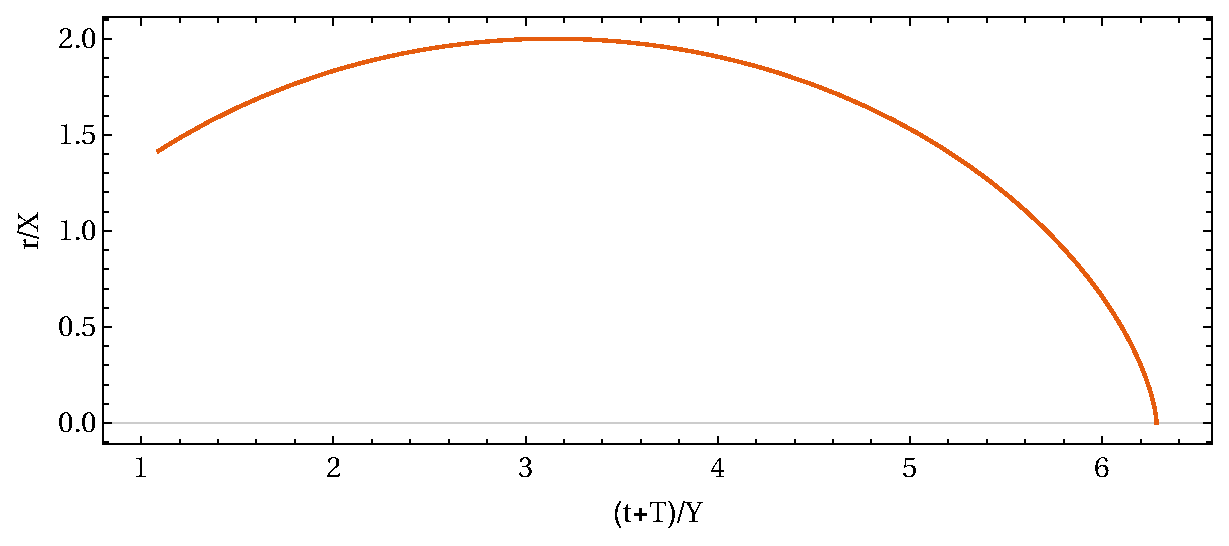
\includegraphics[width=0.7\textwidth]{spherical.eps}
		\caption{\footnotesize Evolution of a spherically overdense region.}
		\label{fig:sphere-cycloid}
	\end{figure}
	Of course, collapse stops before $r=0$ because of pressure generated by fluid. The system \textbf{virializes} and comes to a halt at $r=r_{max}/2$ with a density of $170\rho_b(t_{coll})$ in a matter dominated universe. 
\end{frame}
\subsection{Press-Schechter formalism}
\begin{frame}{Press-Schechter formalism}
	The PS formalism estimates the number of objects collapsed within a mass range of $[M,M+\delta M]$ at a given redshift.
	\begin{block}{Press-schechter mass distribution}
		\begin{equation}
		\frac{dn}{dM}=-\sqrt{\frac{2}{\pi}}\frac{\rho_m}{M}\frac{d\sigma}{dM}\frac{\delta_c}{\sigma^2}e^{\delta_c^2/2\sigma^2}
		\end{equation}
	\end{block}
	\begin{itemize}
		\item $\rho_m/M$ is the average number density of objects of mass M.
		\item $\sigma$ is the variance of the linear power spectrum of density perturbations smoothed by a window function.
		\item $\delta_c$ is the initial critical over-density above which non-linear collapse happens. This is generally taken to be 1.686 
	\end{itemize}
\end{frame}
\section{Data Analysis}
	\subsection{Observed clustering}
		\begin{frame}{Observed clustering}
			\begin{columns}
				\begin{column}{0.35\textwidth}
					\begin{itemize}
						\item Data of over 30,000 QSO sightlines taken from SDSS.
						\item Counted pairs along LoS in redshift space as a function of velocity separation.
						\item Calculated the expected histogram from current model of redshift space distribution.
					\end{itemize}
				\end{column}
				\begin{column}{0.6\textwidth}
					\begin{block}{Completeness correction}
						\begin{itemize}
							\item Surveys tend to report less objects than there are simply because of sensitivity limitations.
							\item Used data from MC simulations by G.B. Zhu to correct for this. 
						\end{itemize}
					\end{block}
				\end{column}
			\end{columns}
		\end{frame}
		\begin{frame}{Observed clustering}
			\begin{figure}
				\includegraphics[width=0.7\textwidth]{MgII_2.pdf}
				\caption{\tiny A comparison of theoretical and observed histograms of pairs of Mg II absorbers. The theoretical estimate has been obtained from the empirical distribution of absorbers in  Zhu \& Menard, The Astrophysical Journal, 770:130 (15pp), 2013 June 20}
				\label{fig:cluster}
			\end{figure}
		\end{frame}
		\begin{frame}{References}
			\begin{enumerate}
				\item \textbf{Zhu, Menard},\textit{The JHU-SDSS Metal Absorption Line Catalogue}, The Astrophysical Journal, 770:130 (15pp), 2013 June 20
				\item \textbf{Nestor, Turnshek \& Rao}, \textit{Mg II absorption systems in SDSS QSO spectra}, The Astrophysical Journal, 628:637–654, 2005 August 1
				\item \textbf{T. Padmanabhan}, \textit{Structure formation in the universe}, Cambridge 1993
				\item \textbf{Jim Peebles}, \textit{Large Scale Structure of the Universe}, Princeton 1992
				\item \textbf{Peter Schneider}, \textit{Extragalactic Astronomy and Cosmology}, Springer 2006
			\end{enumerate}
		\end{frame}
\end{document}